\documentclass[11pt,a4paper]{article}
%\usepackage[utf8]{inputenc}
%\usepackage[ascii]{inputenc}
\usepackage{geometry}
\usepackage[dvipsnames]{xcolor}
\usepackage{textcomp}
\usepackage{graphicx}
\usepackage{caption}
\usepackage{subcaption}
\usepackage{amsmath}
\usepackage{tikz}

\begin{document}

\tableofcontents

\section{Introduction}
This note aims at providing a fresh methodological start in the scope of the DIP2G project. The 6 first months of work on the modelling side of the project can be divided in two roughly equal parts: 1) review of available modelling tools and their achievements. 2) review of the available experimental data on diffuse intrinsic pontine glioma(DIPG) and other glioma cancer cell lines in order to feed  the prospective model. Pages of text have been written on those two subjects before and brief summaries of both will be given in the following paragraphs 

In terms of modelling tools available, the variety of tools makes it difficult to classify them into clear cut categories. Continuous models that tend to treat tissues(i.e cells and their microenvironment) as interacting concentration fields have been used to recapitulate growth dynamics and derive governing equations. Those can be stochastic on deterministic but generally leave out the intracellular scale to focus on "cell-to-tissue"-scale descriptions. On the other end of the spectrum lie models inspired more by systems biology  and that will attempt to recapitulate entire regulation pathways or metabolic fluxes. But of course, representing  all models as belonging to a single axis that would describe scale would be reductive. Several approach can be employed for a given scale. For example, the growth dynamics of spheroids have been replicated both by continuum models of interacting concentration fields and by agent-based models. Agent-based model are best illustrated by "Game of Life" type of simulation where individuals/agents/cells will multiply and interact according  to set rules giving rise to possible emerging properties which are harder to capture with more straightforward mathematical models. A common feature in many of these models is that they require at least some degree of adjustement of  their constants to experimental data. The predictive value of these models often depends strongly on how said fitting is performed.[examples ?] This is not a problem and  a wide array of studies showcase the implementation of the evermore complete models leading to refined behaviors and possible interpretations.

On the biological and experimental side of things, most work on DIPG cell lines is less than two decades old due to inavailability of tractable cell lines beforehand. Several studies have since been performed on different cell lines both in vitro and in vivo with xenograft performed in rats. However, physicists and biologists do not work with and reflect on the same "objects". Physicists will tend to think of tissues and their behavior as a "simple" interplay of nutrients leading to more or less growth in the tissue. Biologists will, for the most part, approach tissue and cell behavior through the study of regulatory pathways which will of course depend on the presence of nutrients but are so interconnected that it is difficult to formulate any prediction to a given change in input. The interconnectedness of different pathways also means that even a slight change in experimental conditions can give results that would be considered completely different by a physicist. Striking examples include how a cell line may "reverse" the citric acid cycle from oxydative phosphorylation to reductive carobyxlation under certain circumstances, The significant difference in oxygen consumption in a given cell line when it is grown as a sphere or as an adherent monolayer, or the different in glycolysis in two apparently close cell lines.

This far, the authors of this study are not interested in sampling 100,000 metabolic flux configurations or testing tens of different hypotheses on larger scale models. Said approach is interesting when the experimental data is readliy available and that one wishes to study possible mechanisms underlying the observed behavior, which is not the case of the DIPG project at the time when those lines are being written. The best approach now, with regards to the available experimental data is to try to answer simple physical question in well-defined configurations and explore the possible implications by looking both at available data and the obtained physical results. The first question that will be adressed in the study is the question of hypoxia.

\section{Hypoxia in DIPG : Quantitative aspects and cell response}
\subsection{A definition of hypoxia}
Diffuse intrinsic pontine glioma are known to be hypoxic tumors.\cite{Bailleul2021} It is in this case necessary to try to define hypoxia both from physical (read "quantitative") and biological point of view. For this purpose, the 2014 review of McKeown provides a good starting point.\cite{McKeown2014} She defines a spectrum of sate corresponding to different levels of oxygenation. Most notably, she outlines the following definitions: 
\begin{itemize}
\item physiological hypoxia : the lower level at which normal hypoxic responses are elicited (range: lower limit approximately 1\%; upper limit possibly $\approx$ 5\%)
\item Pathological hypoxia : shows persistence of poor oxygenation suggesting disruption to normal homeostasis.
\end{itemize} 
In short, physiological hypoxia seems to define a level where the cell can adapt its oxygen consumption in order to maintain oxygen pressure at its physioxic/homeostatic level. While pathological hypoxia seems to define the range for which it becomes impossible for the cell to maintain the oxygen level and therefore homeostasis. This definition already evidences the complex nature of the phenomenon, as it implies that in some cases, the cell can lower their consumption in order to keep the oxygen pressure at given level. Modelling such response would imply knowledge of two things, the different thresholds triggering said response, and the temporal dynamics of it in order to know if any rebound effects are to be included. It should be noted that in general, studies that are referring to hypoxia generally refer to pathological hypoxia with level generally around or below 1\%. \cite{Bailleul2021}\cite{Waker2018}\cite{Saxena2019}

These quantitative aspects leave aside an important aspect of hypoxia and how it impacts cells and tissue : time. Indeed hypoxia, will also be divided into different categories depending on how long the state of hypoxia lasts. "Acute hypoxia" refers to hypoxia that lasts up to 24 hours while hypoxia lasting longer will be referred to as "chronic hypoxia", which may be counterintuitive for the unsuspecting public. Lastly, Chronic hypoxia is defined as a succession of acute hypoxia state followed by reoxygenations. These definitions are not arbitrary and stem from molecular observation about hypoxia. As explained : "Under hypoxia, PHD is inhibited such that HIF-$\alpha$ is not recognized by VHL and hence accumulates"\cite{Saxena2019} and "HIF-1$\alpha$ is ubiquitously expressed, while HIF-2$\alpha$ expression is more tissue specific and expressed in blood vessels, kidney, liver, pancreas, heart, lungs, intestine, and brain". Therefore, initial interest in HIF-1$\alpha$ and HIF-2$\alpha$ will be required in this study. Hypoxia-Inducible Factors are therefore considered the markers of hypoxia in tissue and notably in cancer tissues, and they trigger several cascade that will impact cell behavior in terms of metabolism, proliferation and migration among other things.

This interplay between HIF-1$\alpha$ and HIF-2$\alpha$ seems to be coordinated in a rather widespread fashion across various cell lines : it has been demonstrated in vitro among several endothelial cell line with 0.9 \% O$_2$\cite{Bartoszewski2019},  it was also verified in neurobalstoma cells in vitro at 1\% O$_2$.\cite{Holmquist2006} Said switch was also observed on U87 glioma cells.\cite{Koh2011} In that case, it is interesting to note the difference of response between 0.5 \% O$_2$ and 1\% O$_2$. At 1\% O$_2$ HIF1-$\alpha$ is detectable after 72 hours but has decreased significantly compared to earlier levels while HIF2-$\alpha$. below 0.5 \% O$_2$, HIF1-$\alpha$ decreases notably after 16 hours. In both cases HIF2-$\alpha$ seems to follow HIF1-$\alpha$ and does not (to the author eyes) demonstrate a significant difference in expression in terms of timing. A study on neuroblastoma cell lines demonstrated a more evident shift, but in that case what is shown is that acute hypoxia (at 5\%, 2\% and 1\%) triggers important HIF1-$\alpha$ expression, with mild HIF2-$\alpha$ at 1\% and 2\%.\cite{Lin2011}. Chronic hypoxia (decreasing level with 72 hours steps between each) triggered much more significant HIF2-$\alpha$ expression and much less HIF1-$\alpha$ expression than in the acute case.\cite{Lin2011} It is possible that in the previous case exposition to hypoxia was not long enough to really trigger expression of HIF2-$\alpha$ seen in the latter, if the potential difference between cell line is left out.

Broadly, acute hypoxia (up to 72 hours) seems to trigger expression HIF1-$\alpha$ preferentially, while HIF2-$\alpha$ stabilizes much more after longer period (more than 4 days) of hypoxia around 1\%. Of course duration and relative levels will depend on the cell lines and the severity of hypoxia. The next step is thus to try and gather available data on hypoxia in DIPG cell lines.
  
\subsection{Available data on hypoxia on DIPG}
\subsubsection{Response of DIPG cells to Hypoxia}
The goal of the literature survey performed here is to assess the amount and the kind of data available on hypoxia DIPG cell lines. Our goal is mostly to find data on the expression of HIF1-$\alpha$ and its potential consequences on cell proliferation migration and metabolism. A review from Shen and collaborators reports that when analysing hypoxia, the fact that some cell lines express HIFs constitutively regardless of oxygen levels should be taken into account.\cite{Shen2020} For the cell lines studied in the DIP2G project (DIPG-007 and DIPG-0013)a small expression of HIF1-$\alpha$ is detected on DIPG-007 at 21 \% O$_2$ cultured as adherent monolayers, and this expression goes up signficantly when $pO_2$ is lowered to 1\%\cite{Bailleul2021}. In their study, Waker and collaborators exposed DIPG-IV and DIPG-XIII to hypoxia both "naturally" and through the use of CoCl$_2$.\cite{Waker2018} They report :"All three DIPG cultures retained stable expression of HIF1-$\alpha$ and HIF2-$\alpha$ protein at ambient oxygen tension, unchanged by [hypoxia-mimetics] treatment." What can be noted is that DIPG-IV cells have lower but significant constitutive expression of HIF1-$\alpha$ and HIF2-$\alpha$ than DIPG-XIII. After (supposedly) 24 hours of exposition to 100 \textmu M CoCl$_2$, HIF1-$\alpha$ expression is unaffected in both cell lines. For HIF2-$\alpha$, There is an increase for DIPG-IV and no clear effect for DIPG-XIII. These changes have also been reported for 2\% oxygen level (supposedly) for 24 hours. An interesting fact is that Hexokinase II (glycotlytic enzyme) is strongly expressed in both cell lines with hypoxia compared to control and more so  in DIPG-XIII whose HIFs level do not change with CoCl$_2$. The increase in glycolytic enzyme is coherent with the increase in glycotytic rate increase induced by hypoxia. Another interesting results is that oligomycin which shuts down ATP synthase does not lead to more glycolysis suggesting that these cells do not compensate loss of mitochondrial ATP by up regulating glycolysis(or that they did not have time to do so). Lastly Hypoxia mimetics halted proliferation in both cell lines.

Now there can be an attempt at building a broader picture of the hypoxia response of DIPG cell lines. In normoxia, cells can express more or less constitutive HIFs. Interestingly this may stem from the kind of histone mutations the cell line is associated with DIPG-007 harbor H3.3 mutation while DIPG-4 harbor H3.1 mutation.\cite{Katagi2021} It would be interesting to know if this plays a role into determining HIFs constitutive expression. It will not be easy to conclude on this.

\begin{table}[h]
\begin{center}
\begin{tabular}{ |p{18mm}|p{18mm}|p{18mm}|p{18mm}|p{18mm}|p{18mm}|p{18mm}| }
\hline
\textbf{Cell line} & HIF1-$\alpha$ const. expr & HIF2-$\alpha$ const. expr & HIF1-$\alpha$ hypox. incr. & HIF2-$\alpha$ hypox. incr. & Mutations & Ref \\
\hline
\textbf{SU-DIPG-IV} & Yes & Yes & No & Yes & H3.1K27M ACVR1 & \cite{Waker2018} \\
\hline
\textbf{HSJD-DIPG-007} & Yes & N.D & No & N.D & H3.3K27M ACVR1 &\cite{Bailleul2021} \\
\hline
\textbf{SU-DIPG-XIII} & Yes & Yes & No & No & H3.3K27M TP53 & \cite{Waker2018} \\
\hline
\textbf{HSJD-DIPG-0013} & No & N.D & Yes & N.D & H3.3K27M TP53  & \cite{Bailleul2021} \\
\hline
\end{tabular}
\end{center}
\end{table}

If the focus is put on the two cell lines with the same mutations results are inconsistent with one expressing HIF1-$\alpha$ constitutively while the other does not. The main difference between 0013 and XIII lines is their respective STR profile and culture conditions not being fully detailed by Waker and collaborators. It is possible that Waker and collaborators cultured their cells as monolayers while the DIPG-0013 results presented by Bailleul and collaborators were obtained on cells cultured as neurospheres. Most notably, 96 hours of culture of the DIPG-XIII as neurospheres presented no difference at 21 \% $pO_2$ and 1 \% $pO_2$\cite{Bailleul2021}, while the hypoxia mimetics completely stopped growth for the same duration in the study of Waker and collaborators.\cite{Waker2018} This maybe due to the different culture configuration.

\subsubsection{Oxygen consumption of DIPG cells}
In order to know the extent of hypoxia the cells are subjected to, it is important to know the oxygen consumption of the cells in culture. In most cases, the oxygen consumption rate is measured in monolayers through the use of the seahorse XF kit.\cite{RomeroAgilent} Value are generally reported in pmol/min/cell. Conversion from pmol/cell to mM requires knowledge of the cell volume. a cell volume of 2 pL is postulated (after observation of the picture given by L.), corresponding roughly to a cell diamter of 15 µm which translates into 1.5 mM/min for oxygen consumption. In the case of Mbah and Shen, it was reported in a monolayer-like situation as the cells were plated in wells coated in laminin.  Jiang and collaborators also reported on lung cancer cells that oxygen consumption increased in the monolayer situation compared to the spheroid. This is the first quantitative data we found on that matter and they show OCR to be reduced by two thirds in spheroid compared to monolayers.\cite{Jiang2016} The value for OCR is not to be adjusted as we consider that the contact with the HA/matrigel scaffold produces similar effect to the laminin-coated surfaces used by Shen, Mbah and their collaborators to assess the OCR with the seahorse experiments.

The value reported by Shen and collaborators is 4000 pmol/min/$10^6$ cells which corresponds to a consumption of 2 mM/min/cell. This value is reported for HSJD-DIPG-007 cell line cultured as neurospheres.\cite{Shen2019} In the case of Mbah and collaborators, they derived two models from the HSJD-DIPG-007 and SU-DIPG-XIII cell lines: one grown as neurospheres and another cultured as adherent monolayer with serum. The OCR and ECAR were measured in both cases. For HSJD-DIPG-007 the OCR value reported for gliospheres-cultured cells reported is 50 pmol/min/cell. The first thing is to compare this to the value reported by Shen and collaborators which is 0.004 pmol/min/cell. This means that the same experiment on the same cell line yielded results different by 4 orders of magnitude. Other values reported for brain tumor cells by Ruas and collaborators are in the range of 80 pmol/s/$10^6$ cells, which corresponds to 4800 pmol/min/$10^6$ cells measured in suspension on U87 glioma cells. This is much closer to the value of Shen and collaborators. A possible explanation is a conversion error by Mbah and collaborators. If the value reported by Mbah and collaborators is taken not to be 50 pmol/min/cell but 50 pmol/sec/$10^6$ cells then it becomes much closer to the other values. And to further support this point, the results on ECAR are suggested to the same discrepancy and can be corrected in the same way. Now, if the correction is applied to the gliosphere values for HSDJ-DIPG-007 the measured OCR is 50 pmol/s/$10^6$ cells, which corresponds to 3000 pmol/min/$10^6$ cells, and therefore 1.5 mM/min/cell (assuming a 2 pL cell volume). The same operation for SU-DIPG-XIII yields 4.5 mM/min/cell.

\subsubsection{Incorporating data into the model}
Now that all the information available has been presented, the model will be built by selecting the most relevant aspects. First of all, it is interesting to note that the DIPG cell line with the most available information is the "13" group (i.e. SU-DIPG-XIII and HSJD-DIPG-0013) which harbors the H3.3K27M and TP53 mutations (according to cellosaurus) 

In terms of response to hypoxia those cell line appear  to react as follows. When grown as sphere hypoxia in the range of 1\% $pO_2$ has no noticeable effect on growth over 4 days of the HSJD-DIPG-0013 line. However, the SU-DIPG-XIII line when culture on laminin coated (supposition from the information available in Waker and collaborators poster \cite{Waker2018}) show complete growth arrest when suggest to hypoxia mimetics which should emulate hypoxia in the range of 1-2 \% over the same time period. 

Even though, these situations are most likely not strictly equivalent due to the different type of extracellular matrix proteins being involved (laminin vs. hyaluronic acid), it will nonetheless be assumed that the modelled cells in the matrix should behave like the SU-DIPG-XIII cells in the experiments of Waker and collaborators. This means that cells will undergo growth arrest  below 2\% oxygen pressure.

In terms of oxygen consumption consumption, since an OCR is available for SU-DIPG-XIII on a laminin-coated plate, this value (4.5 mM/min/cell) will also be used in the model. Even though it has been reported that cells may lower their oxygen consumption when oxygen level drops this effect will not be included at first. Therefore this model shall only describe the situation of pathological hypoxia described by McKeown. This may slightly impact the temporal dynamics of the whole system by producing a shorter gradient than in reality. This hypothesis shall be tested later.

A last aspect that will not necessarily be treated right away but should be mentioned here is the impact of glycolysis rate. Indeed it was also measured  on the SU-DIPG-XIII that glycolysis rate increased roughly two-fold when exposed to hypoxia-mimetics for 24 hours. While this does not immediately matter as the model focus solely on oxygen this may strongly impact the glucose dynamics in the model when they are included.

\section{The Tumor-on-chip device and its computational representation}
\subsection{The tumor-on-chip device}
In the scope of the DIP2G project, the most interesting configuration to model is the "tumor-on-chip" configuration. This chip is made of circular well of 10 mm diameter and 750 \textmu m thickness, connected to a microfluidic device through small inlet/outlet holes, as shown in the following drawing.

\vspace{1cm}
\hspace{2cm}
\begin{tikzpicture}
	%inlets
	\draw(0,-0.5) arc(270:90:0.5);
	
	\draw(0,0.5) -- (1,0.5);
	\draw(0,-0.5) -- (1,-0.5);
	
	\draw(8,0.5) arc(90:-90:0.5);
	
	\draw(7,0.5) -- (8,0.5);
	\draw(7,-0.5) -- (8,-0.5);
	
	% center 
	\draw(4,0) circle (3);
	
	%annotations 
	\draw[<->](1.1,0) -- (6.9,0);
	\draw(4,0.5) node {10 mm};
	
\end{tikzpicture}

The circular central part is filled with fluid between two parallel glass blades and also contains the cell/matrix pellet. This pellet is made of a 80/20 mix of Hyaluronic acid, which is the main constitutent of the extracellular matrix (ECM) in the human brain, and matrigel, which is made of the membrane matrix secreted by Engelbreth-Holm-Swarm mouse sarcoma. The proportion is chosen in part to ensure reticulation fast enough to avoid cell sedimentation an maintain them in a 3D configuration.

This information about the matrix composition are important for the following reason: The cross-linking process makes the finalsize of the pellet   variable. Pellet diameter can vary between 4.5 mm and 8 mm depending on experimental parameters. For this reason, in the simulations, the extreme cases of a large and small chip will be treated.

\subsection{The question of fluid circulation}
Another important aspect is the fluid surrounding the pellet in the chip. The volume of fluid in the central part of the chip is more important if the pellet is smaller. This becomes relevant if the chip is used in the non-circulating configuration. In that configuration fresh medium is not circulated continuously in the chip and therefore, glucose, oxygen and other nutrients in the medium deplete over time because of cellular consumption. This means that a larger pellet consumes more and has less reserves than a smaller one.

In the model, the simpler "circulating" configuration will be considered at first. The main reasons being that circulating configuration is approximated in the model by a constant concentration of nutrients in the medium. This is simpler both in terms of programming and in terms of physics. Indeed, with the depleting configuration the cells in the chip never reach a steady state which makes analysis more difficult. In the case of circulating configuration, once the diffusion and consumption have relaxed, the concentration at any point in the pellet is constant and a function of where the considered point lies in the chip.

\subsection{Modelling the chip}
\subsubsection{Geometry and initialisation}
The chip is modelled in MATLAB/Octave using a finite difference algorithm. The spatial step is set a 15 \textmu m which is considered to be theh cell diameter for the studied cell type. Since the reaction-diffusion equation is solved on that grid with an explicit scheme, the time step is set to 1/1500 th of minute the respect the Courant-Friedrichs-Lewy stability condition which depends on the diffusion coefficient of oxygen.\cite{Press1992}

Before going into more detail it should be mentioned that although the situation is 3-dimensional, the representation in the model limits itself to the 2-dimensional circular midsection of the chip. That is to say the 15 \textmu m layer in the middle of the chip. This is justified by several different factors. The system extension along the z-axis is sufficiently large so that translational invariance along that axis can be considered to hold true.  

The grid is a 667x667 square, and a circular domain with the diameter of the pellet is delimited within the square. In order to place the cells within the grid the following way: only non-adjacent grid spots are open for cells. For example if the grid spot at the center of the circular zone corresponding to the pellet is tagged as "open", then the 8 adjacent spots are taken out of the selection. Once all the open spots have been designated, the algorithm randomly fills them with the corresponding number of cells.

 The number of cells is calculated by multiplying the targeted concentration (typically 10 000 cell per \textmu L) by the modelled pellet volume which, in this case, is 15 x $2 \pi r_{pellet}$. As said before the pellet radiusu which has been said to be variable. However it has been said that it is the cross-linking process that reduces the pellet size. It it therefore assumed that all pellets are seeded at a diameter of 8 mm.
 
Lastly is in order to save computational resources those calculations are in fact only performed on a quarter of the grid. The underlying assumption that the axial symmetry in x and y means that the only difference would be the position of certain cell, of which the global density does vary much over the surface of the pellet.

\subsubsection{Modelling Oxygen diffusion and consumption}
Oxygen dynamics within the chip are modelled with the reaction-diffusion equation :

\[ \frac{\partial [C](x,y,t)}{\partial t} = \overrightarrow{\nabla}(D_C(x,y)) \cdot \overrightarrow{\nabla}( [C](x,y,t)) + D_C(x,y,t) \nabla^2 [C](x,y,t) -k_C(x,y,t) \] 

The first diffusion term of the equation is taken as zero in the case of oxygen. Indeed, since the concentration outside the pellet is kept constant, the only diffusion that matters is that within the pellet where the diffusion coefficient is considered constant. The value of diffusion coefficient of oxygen in tissue is taken to be 120000 \textmu m$^2$/min in tissue, which is close to the value used in previous modelling studies on spheroids\cite{Mao2018}\cite{Kempf2015} and close to value measured on agarose gels.\cite{McCabe1975}\cite{Figueiredo2018}.

The consumption term is taken to be in the form of a Hill function of the oxygen concentration : 

\[ k_C(x,y,t) = \frac{[C]^n}{[C]^n + [C]^n_{0}}k_{max}  \]

This function has been used in previous studies to model oxygen consumption. \cite{Mao2018}\cite{Kempf2015}\cite{Jagiella2016}. The $k_{max}$ is the maximum consumption value. The $[C]^n_{0}$ is the concentration value for which the consumption is half of the maximum value. The $n$  exponent is a value that changes the behavior of the function from heaviside function (low $n$) to a sigmoid function (high $n$). As in the models taken for reference, the value for $n$ will be 1 in the model. The value for $[C]^n_{0}$ was taken to be 0.00133 mM by Mao and collaborators and 0.031 mM by Jagiella and collaborators.\cite{Mao2018}\cite{Jagiella2016} The 0.03 mM will be chosen as it was fitted to experimental data rather assumed. The $k_{max}$ value will be taken to be 4.5 mM/min as explained in the previous section. 


\section{Modelling oxygen dynamics in the chip}
\subsection{Results}
The simulations were run for 10 minutes with all the parameters given previously. In figure \ref{DG_map}, the map of cell positions is given for two different pellet size.  \\

\begin{figure}[ht!]
	\begin{subfigure}{0.45\textwidth}
	\centering
	\includegraphics[scale=0.425]{/home/antony/Documents/Post-doc/test_fortran/plots/GO/cfsys2DGO_DG_conf1.pdf}
	\caption{ \label{DG_conf1}}
	\end{subfigure}
	~~
	\begin{subfigure}{0.45\textwidth}
	\includegraphics[scale=0.425]{/home/antony/Documents/Post-doc/test_fortran/plots/GO/cfsys2DGO_DG_conf2.pdf}
		\caption{ \label{DG_conf2}}
	\end{subfigure}
	\caption{Map of the cell localisation in the simulated quarter slice of the tumor-on-chip device for a pellet diameter of 8 mm (a) and 4.5 mm (b). Cells are in blue while the matrix/medium is yellow \label{DG_map}}
\end{figure}
	
The next interesting quantity to follow is the evolution of oxygen in time to assess the temporal relaxation of the system. In figure \ref{Ot}, it can be seen that the system relaxes in less than 2 minutes, which could be expected given the diffusion coefficient of oxygen and the max consumption value in the study. It should however be noted that this short time of relaxation correspond to the extracellular dynamics of oxygen dictated by physics, which are not equivalent to the response time of cells to the external stimulus which is most likely longer.\\
 
\begin{figure}[ht!]
	\begin{subfigure}{0.45\textwidth}
	\centering
	\includegraphics[scale=0.425]{/home/antony/Documents/Post-doc/test_fortran/plots/GO/cfsys2DGO_Ot_conf1.pdf}
	\caption{ \label{Ot_conf1}}
	\end{subfigure}
	~~
	\begin{subfigure}{0.45\textwidth}
	\includegraphics[scale=0.425]{/home/antony/Documents/Post-doc/test_fortran/plots/GO/cfsys2DGO_Ot_conf2.pdf}
		\caption{ \label{Ot_conf2}}
	\end{subfigure}
	\caption{Time evolution of the oxygen concentration for for a pellet diameter of 8 mm (a) and 4.5 mm (b) at the rim and center of the pellet. \label{Ot}}
\end{figure}

Finally, one should look at the concentration maps of oxygen in the relaxed system which are displayed in figure \ref{O_ctrmap}. It can be seen that the steady-state oxygen gradient resulting from the balance of diffusion and consumption. In the case of the 8 mm wide pellet, the gradient is slightly above 600 \textmu m while it is closer to 400 \textmu m in the case 4.5 mm wide pellet. In both cases, large central portions of the chip have a zero concentration of oxygen. This will be the next extension of this study.

\begin{figure}[ht!]
	\begin{subfigure}{0.45\textwidth}
	\centering
	\includegraphics[scale=0.425]{/home/antony/Documents/Post-doc/test_fortran/plots/GO/cfsys2DGO_O_ctr_conf1.pdf}
	\caption{ \label{O_ctr_conf1}}
	\end{subfigure}
	~~
	\begin{subfigure}{0.45\textwidth}
	\includegraphics[scale=0.425]{/home/antony/Documents/Post-doc/test_fortran/plots/GO/cfsys2DGO_O_ctr_conf2.pdf}
		\caption{ \label{O_ctr_conf2}}
	\end{subfigure}
	\caption{Contour map of the oxygen concentration for for a pellet diameter of 8 mm (a) and 4.5 mm (b) at the rim and center of the pellet. \label{O_ctrmap}}
\end{figure}

The scale in the contour map has been rescaled to have "saturate" at 0.015 mM (2\%). The darkest line correspond to an oxygen level of 0.002 mm ($\approx$ 0.2\%). The yellow part therefore correspond to the area of the pellet where cells are not in physiological hypoxia. All cells beyond that point should be considered to express more HIF1-$\alpha$ and/or HIF2-$\alpha$ than the ones on the rim according to the data gathered by Waker and collaborators. Another intersting observation in this study is that SU-DIPG-XIII cells subjected to hypoxia stopped their proliferation and raise their glycolytic rate two-fold.\cite{Waker2018} Including glucose consumption and this glycolytic increase in the model will be the core of the next study. 

\subsection{Discussion}

\section{Model with glucose consumption}
\subsection{Modelling glucose dynamics}
The glucose consumption in the model is handled in a similar way to oxygen consumption, that is to say, using a reaction-diffusion equation and a Hill  function to model the evolution of consumption as a function of nutrient availability.

\subsubsection{Glucose diffusion}
This means that values for parameters of diffusion and the consumption are needed in order to perform the simulations. As for oxygen, the glucose outside the pellet is considered to be constant in time and space. Therefore, the only diffusion coefficient needed is that of glucose in matrix and tissue. Indeed, the concentration of cells is important but they are not as tightly packed as they would be in a spheroid. It seems sensible to assume that the effective diffusion coefficient for glucose in that configuration will be lower than that of a pure Hyaluronic acid/matrigel gel and higher than that of a densely packed tissue made of cells and the same matrix

Literature review did not provide a glucose diffusion value human brain tumors. However, a study from 1982  by Li measured a glucose diffusion coefficient of $1.5\cdot 10^{-6}$ cm$^2$/s (9000 \textmu m$^2$/min) for 9L rat brain tumor spheroids.\cite{Li1982} For lack of data closer to the model used in this study, this will be taken as the "packed tissue" value. 

For the pure matrix value, the results for glucose diffusion in Hyaluronic acid gels in PBS are less straightforward. Indeed, a study from Hadler showed that glucose diffusivity ranged between $0.8\cdot 10^{-5}$ cm$^2$/s and $0.5\cdot 10^{-5}$ cm$^2$/s for concentration of 0.5 \% and 1 \%, but increases to $2.0\cdot 10^{-5}$ cm$^2$/s for concentration of 2.5\%, which is in the range of concentrations used in physiological studies with hydrogels.\cite{Gerecht2007} Therefore, in the model both the normal and enhanced glucose diffusion cases will be treated.

To adress the question of chip not being pure matrix, an estimation of tortuosity can be made. Tortuosity is defined as either the ratio of effective and free diffusion coefficient, the ratio of the square of the previous quantities, the ratio of path length of molecules in the porous medium and in free medium, or the square of that quantity. In their study, Hamad and collaborators asess different models that link tortuosity to porosity.\cite{Hamad2018} With an initial concentration of 10 000 cells per \textmu L in the chip, the porosity ranges between 97\% for the large pellet and 0.90\% 

If the models of Maxwell and Berryman are used, the obtained  are comprised between 1.015 and 1.06. Therefore, it will be considered that cells do not significantly impact the diffusion properties, so the values for glucose diffusion are the matrix values : $0.5\cdot 10^{-5}$ cm$^2$/s (low diffusion case) which corresponds to 30000 \textmu m$^2$/min, and $2.0\cdot 10^{-5}$ cm$^2$/s (enhanced diffusion case) which corresponds to 120000 \textmu m$^2$/min.
%0.97 (8 mm)
%0.896 (4.5mm) 

\subsubsection{Glucose consumption}
As for the oxygen the parameters of the Hill function for glucose need to be determined. 

The Hill function exponent is taken as unity similar to oxygen. No clear measurements in a low glucose environment performed on the SU-DIPG-XIII of HSJD-DIPG-0013 cell line have been found in the literature. The hypothesis is made that consumption drops to 50 \% when glucose level falls below 1 mM.

Similar to glucose diffusion, no direct glucose consumption measured have been performed on in vitro cultures of SU-DIPG-XIII or HSJD-DIPG-0013 cells. 
However, measurements have been performed on glioma and glioblastoma cell lines such as GBM39, U251 and A549 cells. In order to progress further these values will be presented and used in this study.

Measurements were usually performed with glucose consumption assay kits and performed on standard 96-well or 6 well plate by plating a density of cells ranging from 10000 to 40000 cells per well. No specific laminin coating are reported and the consumption is generally evaluated by measuring the concentration of glucose after a giving time period (12-24hrs). For all given values, the cells potentially dividing during that period are not accounted for which may make  the value slightly overestimated since they are calculated with the initial cell density.\cite{Mai2017}\cite{Shankland2002}\cite{LiuFM2021}

Measurements performed by Mai and collaborators on the GBM39 cell line yielded a consumption of 0.006 nmol/cell/12hr which in this study's model translate into 4.15 mM/min assuming a cell volume of 2 pL.\cite{Mai2017} Shankland and collaborators reported a glucose consumption of approximately 1 mM over 200 mn for 70 million A549 cells, which translates into 3.8 mM/min following the same conversion as before. Liu and collaborators reported a consumption of 1 mg/mL over 24 hours in U251 (wt) cells, which translates a value of 8.5 mM/min in the model that will be used for this study.\cite{Liu2021}

The scope of values obtained leads to the study of high consumption case (8 mM/min) and a low consumption case (4 mM/min), similar to the case of standard and enhanced diffusion presented in the previous part. 
 

\subsubsection{Hypoxia-induced increase in glycolytic rate}
The results of Waker and collaborators show that the glycolytic rate in SU-DIPG-XIII increased from $\approx$ 120 pmoles/min to $\approx$ 240 pmoles/min when hypoxia-mimetics are induced through 100 \textmu M of CoCl$_2$. While it is not explicitly stated in the document, it can be assumed that the 100 \textmu M concentration of of CoCl$_2$ should correspond to an oxygen level of 2 \%. It is also intersting to note that the glycolytic rate before the addition of glucose are quite close, suggesting that very little acidification comes from mitochondrial metabolism or other sources, notably whein compared to the SU-DIPG-IV cell line.

The increased consumption is included in a straight forward fashion : When oxygen concentration falls below 0.015 mM (2\%), the value of $k_{max,glu}$ is multiplied by 2. It is interesting to note that the consumption of oxygen starts decreasing at 0.03 mM which is above the level where the shift in glycolysis occurs.

\newpage
\subsection{Results on glucose}
As explained before due to the absence of glucose measurements on diffusion and consumption in SU-DIPG-XIII and HSJD-DIPG-0013 cell lines, value for the simulation were taken for other cancer tissue or glioma cell line. Since two "regimes" were identified for pellet size, glucose consumption, and glucose diffusion, all those cases will be treated in the following section in the following order :

\begin{table}[h]
	\begin{center}
		\begin{tabular}{ |p{15mm}|p{41mm}|p{34mm}|p{27mm}|}
			\hline
			\textbf{Config.} & $k_{max,glu}$ (mM/min) & $D_{glu,tiss}$ (\textmu m$^2$/min) & $d_{pell}$ (\textmu m) \\
			\hline
			\textbf{1} & 4 & 30000 & 8000 \\
			\hline
			\textbf{2} & 8 & 30000 & 8000 \\
			\hline
			\textbf{3} & 4 & 30000 & 4500 \\
			\hline
			\textbf{4} & 8 & 30000 & 4500 \\
			\hline
			\textbf{5} & 4 & 120000 & 8000 \\
			\hline
			\textbf{6} & 8 & 120000 & 8000 \\
			\hline
			\textbf{7} & 4 & 120000 & 4500 \\
			\hline
			\textbf{8} & 8 & 120000 & 4500 \\
			\hline
		\end{tabular}
	\end{center}
\end{table}

For each configuration the spatial and temporal dynamics of glucose in the pellet will be discussed. As before, the supply is considered to be constant outside the pellet.

\subsubsection{Configuration 1: Large \& slow}
Configuration 1 correspond to the case of a large pellet in which standard diffusion and low glucose consumption take place. The implemented consumption hike due to hypoxia does work. However, the short relaxation time means the inflexion is barely visible on the graph.

\begin{figure}[ht!]
	\begin{subfigure}{0.45\textwidth}
	\centering
	\includegraphics[scale=0.425]{/home/antony/Documents/Post-doc/test_fortran/plots/GOr/cfsys2DGGr_G_ctr_conf5.pdf}
	\caption{ \label{G_ctr_conf5}}
	\end{subfigure}
	~~
	\begin{subfigure}{0.45\textwidth}
	\includegraphics[scale=0.425]{/home/antony/Documents/Post-doc/test_fortran/plots/GOr/cfsys2DGOr_Gt_conf5.pdf}
		\caption{ \label{Gt_conf5}}
	\end{subfigure}
	\caption{\textbf{Configuration 1:} Contour map of the glucose concentration for a pellet diameter of 8 mm (a) Time evolution of the glucose concentration at the center and ath the rim of the pellet (b). \label{G_t_ctr_1}}
\end{figure}

This is the "slowest" configuration in terms of relaxation time. This is due to the large size of the system, slow diffusion and relatively low consumption. As can be seen in figure \ref{G_t_ctr_1}, the system relaxes to a minimal value of 0 at the center in 200 minutes. This also results in that configuration being the most depleted in the center. A close inspection of the glucose profile (not shown) shows that glucose concentration is halved roughly 1000 \textmu m-deep into the chip in this configuration and that complete depletion occurs at 3000 \textmu m depth.

\newpage
\subsubsection{Configuration 8 : Small \& fast}
Configuration 8 is the polar opposite of configuration 1. In that case, diffusion is fast, consumption is high meaning the system equilibrates quickly. The pellet size is also the smallest observed.

\begin{figure}[ht!]
	\begin{subfigure}{0.45\textwidth}
	\centering
	\includegraphics[scale=0.425]{/home/antony/Documents/Post-doc/test_fortran/plots/GOr/cfsys2DGGr_G_ctr_conf12.pdf}
	\caption{ \label{G_ctr_conf12}}
	\end{subfigure}
	~~
	\begin{subfigure}{0.45\textwidth}
	\includegraphics[scale=0.425]{/home/antony/Documents/Post-doc/test_fortran/plots/GOr/cfsys2DGOr_Gt_conf12.pdf}
		\caption{ \label{Gt_conf12}}
	\end{subfigure}
	\caption{\textbf{Configuration 8:} Contour map of the glucose concentration for a pellet diameter of 8 mm (a) Time evolution of the glucose concentration at the center and ath the rim of the pellet (b). \label{G_t_ctr_8}}
	
The system equilibrates in less than an hour at a central value of 5 mM. and this concentration falls to half the external value at approximately 1000 \textmu m depth.
\end{figure}

\subsubsection{Discussion on glucose}
Two extreme cases have been identified based on the spread of experimental values for glucose-related parameters found in the literature on glioma cell lines. In the slow and large case, the chip is fully glucose-depleted at its center after 3 hours. In the fast and small case, the glucose does not fully depleted at the core of the chip but falls at one fifth of the external values.

\subsubsection{Analysis of glucose and oxygen}
Now that the steady-state distribution of glucose and oxygen has been determiend in the two extreme cases, they are presented in figure \ref{GO_x}

\begin{figure}[ht!]
	\begin{subfigure}{0.45\textwidth}
	\centering
	\includegraphics[scale=0.4]{/home/antony/Documents/Post-doc/test_fortran/plots/GOr/cfsys2DGOr_GO_conf5.pdf}
	\caption{ \label{G_ctr_conf12}}
	\end{subfigure}
	~~
	\begin{subfigure}{0.45\textwidth}
	\includegraphics[scale=0.4]{/home/antony/Documents/Post-doc/test_fortran/plots/GOr/cfsys2DGOr_GO_conf12.pdf}
		\caption{ \label{Gt_conf12}}
	\end{subfigure}
	\caption{Steady-state profile of normalised glucose and oxygen concentration in the chip in the "large and slow" case (a), and in the fast and small case (b). The red line delimits the hypoxic zone ([O]<2\%) and the 50 \% mark for glucose concentration. \label{GO_x}}
	\end{figure}
	
The vertical lines are here to represent two limits. In the case of oxygen the threshold was fixated to 2 \% due to the information found in various publication on the subject and specifically the results of Waker and collaborators shown in their 2018 poster.\cite{Waker2018} It delinates the cell that should significantly express HIF1-$\alpha$  and HIF2-$\alpha$ and go into growth arrest. For glucose no known limits for survival or starvation are known so the 50 \% is mostly indicative  but it helps evidence that no matter where the limit lies there will probably a mostly necrotic central area, a mostly quiescent layer and a proliferative layer. However, since the model has focused so far on a maximum timespan of three hours no clear discussion about cell state can be had in this section. This will be the focus of the next part.

\section{Cell growth \& nutrients dynamics in the chip}
In the previous parts, the nutrient dynamics were explored in the chip. As a results of studying both oxygen and glucose dynamics in the constant supply case under certain hypothesis and using experimental values from different sources, it was found that an hypoxic zone could be delimited and that this hypoxic zone itself contained two areas separated by a limit which defines the glucose level leading to cell death. However, the glucose level leading to cell death so far is unknown. The first part of this third study will thus be a literature review aiming at the determination/estimation of such threshold. Once the threshold is set, the next step will be to include the cell cycle and its potential interaction with the environment in order to assess the proportion of dead, arrested and proliferative.

\subsection{Nutrient starvation impact on cancer cells}
Most Cancer cells including brain tumor cell lines display some form metabolic plasticity. Metabolic plasticity is the ability of cells to maintain their energy supply by switching from one substrate or metabolic pathway to another when the environment becomes challenging.\cite{Venneti2016}\cite{DeBerardinis2008}\cite{Spinelli2018} In cancer cells, examples include, increased glycolysis in hypoxic condition or the ability to switch between glucose and glutamine in carbon source.\cite{Waker2018}\cite{Natarajan2019} These adaptation often "aim" at the maintenance of the ATP production rate in the absence of the normal/main supply for a given duration.\cite{Piannet1991}

So far, oxygen and glucose have been included, and the model based mostly on the SU-DIPG-XIII and HSIJD-DIPG-0013 observed behavior in hypoxia. The next question in line was to understand how glucose starvation in the hypoxic zone could lead to cell death. Before going further, it should be noted  that Griguer and colleagues showed that this question is far from trivial. Indeed, "The D-54MG and GL261 glioma cell lines displayed an oxidative phosphorylation (OXPHOS)-dependent phenotype, characterized by extremely long survival under glucose starvation, and low tolerance to poisoning of the electron transport chain (ETC). Alternatively, U-251MG and U-87MG glioma cells exhibited a glycolytic-dependent phenotype with functional OXPHOS. These cells displayed low tolerance to glucose starvation and were resistant to a ETC blocker."\cite {Griguer2005} In this study, it is assumed for now that adaptation of cells to glucose scarcity cannot be remediated through an increase in oxydative phosphorylation. The authors are aware of the fact that hypoxia does not equate to complete ETC impairement, and that the assumption "hypoxia = no ETC function" is simplistic.  This hypothesis is mostly made to limit the scope of the study. 

In light of the previous paragraph, in the model the only possible mechanism for cell in response to a scarcity of glucose is to switch to glutamine as a carbon source. In last resort, cells may also resort to fatty acids oxidation and autophagy as well. None of those will not be explictly  included and will be considered to be encompassed in the delay between glucose and oxygen depletion of the environment and the occurence of cell death due to starvation. The delay will be taken to be 8 hours in accordance to experiments made by Piannet on C6 rat glioma cells.\cite{Piannet1991} While a complete modelling of other nutrients such as glutamine would be more satisfactory, there is not enough quantitative data on the diffusion and consumption of glutamine in chip matrix to be able to provide the same modelling as for oxygen and glucose.


\subsection{The conditions for cell death}
Previous models for spheroid growth have accounted for the cells metabolic plasticity by setting a threshold for cell death that depends on both glucose and oxygen.\cite{Kempf2005}\cite{Jagiella2016} This reflects the fact that cell death in a nutrient based model will be linked to an insufficient ATP production. The question then becomes : what would be a realistic threshold of sufficient ATP production to ensure survival ? An experimental from Lieberthal and collaborators gives interesting information on that subject. Indeed, they report in the abstract of their paper: "We found that cells subjected to ATP depletion below approximately 15 \% of control died uniformly of necrosis. In contrast, cells subjected to ATP depletion between approximately 25 and 70 \% of control all died by apoptosis. The rapidity of cell death was proportional to the severity of reduction of cell ATP content and was independent of the mechanism of cell death."\cite{Lieberthal1998}

The previously mentioned  results were obtained on mouse proximal tubular cells, which are not cancerous, brain or even human cells. This means that, assuming that the same mechanisms apply to brain tumors  the threshold may not be the same depending on cell function. However, other studies seem to suport that the mechanism is widespread at least qualitatively.\cite{Martin2001} The following point of interest is the place of apoptosis in the model. Most agent-based model treating tumor growth do not account for apoptosis, and only include necrosis in their cell death mechanism.\cite{Mao2018}\cite{Kempf2005}\cite{Kempf2015}\cite{Bull2020}\cite{Jagiella2016}\cite{Cleri2019}For the sake of simplicity only necrosis will be considered in this study as well.


\subsection{The importance of cell cycle}
Building on the knowledge presented right before a mechanism of cell death that accounts for the ATP level and the cell cycle phase is proposed here. Cells are considered to be able to survive for 8 hours in a depleted environment. In the model, glucose depletion necessarily occurs in zone that are already hypoxic. In that case, keeping in with the values given by Lieberthal, if it assumed that ATP production is almost completely provided by glycolysis in hypoxic cells then a fall below 25 \% on the external concentration for more than 8 hours should lead to cell death. However the possibility of cell cycle arrest should not be overlooked. Therefore, it is proposed to refine the previous statement slightly by including a dependence on the cell cycle phase: 
\begin{itemize}
\item If a cell is less than 8 hours before division when the glucose concentration crosses the threshold, then the cell survives and goes into growth arrest immediately after division. 
\item If a cell is in G1 phase when the concentration crosses the threshold it stops its growth.
\item If cells is in G2 phase and more than 8 hours before division then the cell dies after 8 hours.
\end{itemize} 

\begin{figure}[ht!]
\vspace{1cm}
\hspace{2cm} 
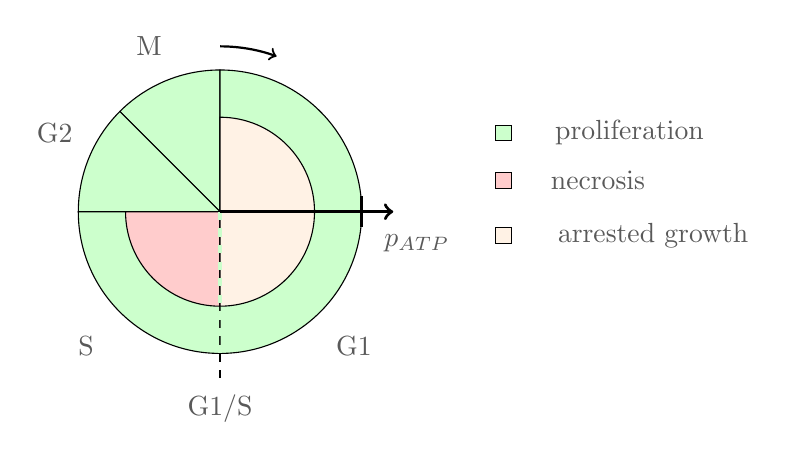
\begin{tikzpicture}


\filldraw[fill=green!20!white, draw=black] (0,0) -- (0mm,18mm) arc (90:135:18mm) -- (0,0);
%\filldraw[fill=red!20!white, draw=black] (0,0) -- (0mm,12mm) arc (90:135:12mm) -- (0,0);
\draw[thick,gray!70!black](-9mm,21mm) node {M};


\filldraw[fill=green!20!white, draw=black] (0,0) -- (-18*0.707mm,18*0.707mm) arc (135:180:18mm) -- (0,0);
%\filldraw[fill=red!20!white, draw=black] (0,0) -- (-12*0.707mm,12*0.707mm) arc (135:180:12mm) -- (0,0);
\draw[thick,gray!70!black](-21mm,10mm) node {G2};

\filldraw[fill=green!20!white, draw=black] (0,0) -- (-18mm,0mm) arc (180:270:18mm) -- (0,0);
\filldraw[fill=red!20!white, draw=black] (0,0) -- (-12mm,0mm) arc (180:270:12mm) -- (0,0);
\draw[thick,gray!70!black](-17mm,-17mm) node {S};


\filldraw[fill=green!20!white, draw=black] (0,0) -- (-0mm,-18mm) arc (-90:90:18mm) -- (0,0);
%\filldraw[fill=cyan!10!white, draw=black] (0,0) -- (18*0.866mm,18*0.5mm) arc (30:90:18mm) -- (0,0);
\filldraw[fill=orange!10!white, draw=black] (0,0) -- (-90:12mm) arc (-90:90:12mm) -- (0,0);
%\filldraw[fill=red!20!white, draw=black] (0,0) -- (9*0.866mm,9*0.5mm) arc (30:-90:9mm) -- (0,0);
\draw[thick,gray!70!black](17mm,-17mm) node {G1};

\draw[draw=green!20!white, dashed,very thick] (0,0) -- (-0mm,-18mm);
\draw[very thick, ->] (0mm,0mm) -- (22mm,0mm);
\draw[very thick] (18mm,2mm) -- (18mm,-2mm);
\draw[thick,gray!70!black](25mm,-4mm) node {$p_{ATP}$};
%\draw[draw=black, thick] (0,0) -- (18mm,10.2mm);
%\draw[thick,gray!70!black](20mm,10.5mm) node {R};
\draw[draw=black, dashed] (0,-18mm) -- (0 mm,-22mm);
\draw[thick,gray!70!black](0mm,-25mm) node {G1/S};


\draw[thick,->] (0mm,21mm) arc(90:70:21mm);
%\draw[dashed] (0mm,-15mm) arc(-90:30:15mm);

%legend
\filldraw[fill=green!20!white, draw=black] (35mm,9mm) rectangle (37mm,11mm);
\draw[thick,gray!70!black](52mm,10mm) node {proliferation};
\filldraw[fill=red!20!white, draw=black] (35mm,3mm) rectangle (37mm,5mm);
\draw[thick,gray!70!black](48mm,4mm) node {necrosis};
\filldraw[fill=orange!10!white, draw=black] (35mm,-2mm) rectangle (37mm,-4mm);
\draw[thick,gray!70!black](55mm,-3mm) node {arrested growth};

\end{tikzpicture}
\caption{Cell fate as a function of ATP production and cell cycle phases \label{cell_fate}}
\end{figure}
In figure \ref{cell_fate}, the previously mentioned behavior has been slightly simplified in order to let the limits of each behavior coincide with a phase of the cell cycle. Cancer cells doubling time can between 18 and a few days, and more specifically between 20h and 30h for glioblastoma.\cite{Oraiopoulou2017} However, this doubling time has been reported to be of the order of 6 days for SU-DIPG-XIII.\cite{He2021} It should be noted that using the data from Waker's poster the estimate for doubling time is closer to 2.8 days rather 6.6. But the culture conditions are not fully known in that case, and the normal oxygen concentration is known to be different between the two studies which may explain the difference. It is also known that if glucose concentration is higher, the doubling time may change.\cite{Casciari1992}\cite{Yang2021} Considering the fact that the model in this study is based mostly on Waker's results and that the external concentration in the model is 20 \% and not five the doubling time of well-nourished cells is taken to be 3 days.

Accounting for the previous paragraph, the next question becomes :"How long is each phase of the cell cycle ?" Is the lengthening of the cell cycle striclty equivalent to G1-phase lengthening, with the G2, M and S phase having constant duration ? Or is every phase of the cell cycle lengthened in a proportional fashion ? The study of Chao and collaborators indicate that among various cell types the G1-phase is the most variable one compared to more G2,S and M phase, which are more consistent across cell lines.\cite{Chao2019} However, the review by Fisher and Krasinska seem to indicate that at least some cell types exhibit the opposite behavior:"In lymphocytes, the duration of all phases varies considerably and is proportional to the inter-division time, with the majority of cell cycle time variability resulting from the combined length of the S/G2/M phase."\cite{Fisher2022}. The answer is that it probably depends both on the cell type and external conditions.

In this model the answer to that question impacts the results. Indeed, with the hypothesis presented previously, cell can only die in a time window situated in S-phase and/or G2-phase. If all phases are lengthened in a roughly equal fashion when cell cycle length varies then the length of the cell cycle does not change the probability for a cell to die or not. However, if phase lengths do not vary equally then the probability for a cell of being in the phase where it can die may diminish with a lengthening cell cycle. This is why it is important to consider both cases.

\subsection{Cell cycle length and different phases}
\subsubsection{Cell cycle length}
First of all, the data presented in Waker's poster and in He and collaborators study give an idea of the variation of the cell cycle duration with oxygen concentration. At 20 \% the SU-DIPG-XIII doubling time can be calculated to be 2.8 days (using the same methods as He and collaborators). In the study of He and collaborators, at 5 \% the doubling time is reported to be 6.6 days on the same cell line.\cite{He2021} This seems coherent as the 5 \% value can be seen as an intermediate between hypoxia and the ambient oxygen level of 20 \%. In hypoxia ($\approx 2$ \%), emulated by addition of 100 \textmu M of CoCl$_2$ in the medium, growth is all but completely stopped.\cite{Waker2018}

Taking into account the previous data, a function linking the observed doubling time on SU-DIPG-XIII and the oxygen concentration can be derived. The function displayed in figure \ref{podbl} is of the form $\frac{a}{b x - c }$ where $a$, $b$ and $c$ were determined with least squares approach. The following values were determined : $a =  13.0612;  b = 0.6694; c = 1.3061$.

\begin{figure}[ht!]
\vspace{1cm}
\hspace{4cm} 
\begin{tikzpicture}[domain=0:4] 
    %\draw[very thin,color=gray] (-0.1,-1.1) grid (3.9,3.9);
    %axes
    \draw[->] (-1.7,0) -- (4.5,0) node[right] {$pO_2$}; 
    \draw[->] (-1.5,-0.2) -- (-1.5,4.2) node[above] {doubl. time};
    
    %ticks
     \draw[-] (0,-0.2) -- (0,0.2);
     \draw (0,-0.6) node {2 \%};
     \draw[-] (4,-0.2) -- (4,0.2);
     \draw (4,-0.6) node {20 \%};
     \draw[-] (1,-0.2) -- (1,0.2);
     \draw (1,-0.6) node {5 \%};
     
     %lines
     \draw[dashed] (0,0.2) -- (0,4.2);
     \draw[dashed] (4,0.2) -- (4,4.2);
     \draw[dashed] (1,0.2) -- (1,4.2);
     
      \draw[domain=0.1:4.3,color=blue] plot (\x,{exp(-2*\x+1.5)+1});
      \draw[domain=0.1:4.3,color=blue] plot (\x,{exp(-2*\x+1.5)+1});
      %\draw[domain=0:3,color=green!30!black] plot (\x,\x);
      %\draw[domain=3:4.3,color=green!30!black] plot (\x,3);
      %\draw[color=green!30!black] (5.5,3) node {$v_{max,GF+}$};
      %\draw[domain=0:3,color=green!60!black] plot (\x,0.5*\x);
      %\draw[domain=3:4.3,color=green!60!black] plot (\x,1.5);
      %\draw[color=green!60!black] (5.5,1.5) node {$v_{max,GF-}$};
  \end{tikzpicture}
  \caption{Relation doubling time, and oxygen partial pressure \label{podbl}}
\end{figure}

Once again, in all fairness the impact of glucose on doubling time should also be determined. But such data is not available on SU-DIPG-XIII. Moreover the physical configuration of the model means that an area where oxygen would be plenty and glucose depleted cannot exist in the model. Therefore so far only oxygen can impact the doubling time. There is not a strict equivalence between doubling time, which is measurement made on a whole culture and cell cycle length, which is a property of the individual cell. In the model, though, the doubling time will be equated to the cell cycle length.

\subsubsection{Length of the different phases}
As explained before, cell cycle phases do not necessarily vary in proportion with the cell cycle length. First of all, it seems to be clear that mitosis duration is an hour at most (including cytokinesis)\cite{Cooper2006}\cite{Araujo2016}\cite{Chao2019} and does not vary when the duration of other phases do.

Even though a first literature review suggested that G1, G2 and S phases may vary independently\cite{Chao2019}\cite{Fisher2022}, a more specific search on the impact of starvation seem to suggest that serum or nutrient starvation leads mostly to G0/G1 phase arrest.\cite{Wang2021}\cite{Chen2012}\cite{Hahn2009} It is thus assumed from this point in the model the only phase that can vary in length is G1-phase. This, however, does not give any information about the respective length of the cell cycle phases in normal conditions.

The best piece of information that was found on that matter in the literature was the respective proportion of patient derived DIPG cells obtained by Sun and collaborators. They reported 80 \% of cells in G1 phase, with 14\% in S-phase and 6\% in G2 phase at low passage and approximately 90 \% in G1, and 5\% in both G2 and S phases.\cite{Sun2019} Assuming that cells are not synchronized, the proportion can be turned into relative length for the cell cycle phases : 
\begin{itemize}
\item Mitosis is an hour long (at most 1.4 \% of total cell cycle length)
\item G2 phase duration will be taken to be 5\% of the whole cell cycle at 20 \% $pO_2$ : 3.3 hours
\item S phase duration will be taken to be 15\% of the whole cell cycle at 20 \% $pO_2$ : 10 hours
\item G1-phase duration will be taken to be 80\% of the whole cell cycle at 20 \% $pO_2$ : 53 hours
\item G1-phase length will evolve concomittantly with the cell cycle length.
\end{itemize}

Since only the G1-phase length changes with $pO_2$, the previous function is refitted to time data where the duration of all phases but the G1-phase are removed. This new fit yielded the resulting coefficients. $a =  17.9592;  b = 0.9816; c = 1.9184$.
  
$a =  0.032594;  b = 5.6239e-07; c = -1.0682e-06$.


\section*{Appendix}
\subsection*{Proof of the validity of the 2D approximation}
\newpage
\bibliographystyle{unsrt}
\bibliography{biblio_synthese}
\end{document}

